\documentclass[a4paper,14pt]{extarticle}

% Шрифты, кодировки, символьные таблицы, переносы
\usepackage{cmap}
\usepackage[T2A]{fontenc}
\usepackage[utf8x]{inputenc}
\usepackage[english, russian]{babel}

% Пакеты американского математического сообщества
\usepackage{amssymb,amsfonts,amsmath,amsthm}  
% Сокращения
\usepackage{cancel}

\theoremstyle{definition}
\newtheorem{definition}{Определение}

% Красная строка
\usepackage{indentfirst}

% Ссылки в pdf
\usepackage[unicode, colorlinks, urlcolor=magenta, linkcolor=black]{hyperref}

% Таблицы
\usepackage{makecell,multirow} 

% Графика
\usepackage{graphicx}
\usepackage[usenames,dvipsnames]{color} 
\usepackage{float}
% \usepackage{subcaption}

% Геометрия страницы
\usepackage{geometry}
\geometry{left=2cm,right=2cm,top=2.5cm,bottom=2.5cm,bindingoffset=0cm,headheight=18pt}

% Колонтитулы
\usepackage{fancyhdr} 
% применим колонтитул к стилю страницы
\pagestyle{fancy} 
%очистим "шапку" страницы
\fancyhead{} 
%слева сверху на четных и справа на нечетных
\fancyhead[R]{Лекции В.И. Некоркина 2018-2019} 
% \fancyhead[R]{Сарафанов Ф.Г., Понур К.А. и др.} 
%справа сверху на четных и слева на нечетных
\fancyhead[L]{Теория колебаний} 
%очистим "подвал" страницы
\fancyfoot{} 
% номер страницы в нижнем колинтуле в центре
\fancyfoot[C]{\thepage} 

% Межстрочный отступ
\usepackage{setspace}
\linespread{1.15} % капельку увеличенный
\frenchspacing % <<французские>> пробелы

% Нумерация
\renewcommand{\labelenumii}{\theenumii)}
% В заголовках появляется точка, но при ссылке на них ее нет
\usepackage{misccorr}

% Содержание
\usepackage{tocloft}
\usepackage{secdot}
\sectiondot{subsection}

% Физика
\usepackage{physics}

% Новые команды
\newcommand{\Mean}[1]{\langle#1\rangle}
\newcommand{\Defi}{\underset{def}{=}}
\newcommand{\Inte}{\int\limits_{-\infty}^{\infty}} 

\addto\captionsrussian{%
	\renewcommand{\contentsname}{Оглавление}
	\renewcommand{\partname}{Раздел}%
}
\def\thepart{\arabic{part}}
\usepackage{tocloft}
\renewcommand{\cftpartleader}{\cftdotfill{\cftdotsep}} % for parts
% \renewcommand{\cftchapleader}{\cftdotfill{\cftdotsep}} % for chapters
\renewcommand{\cftsecleader}{\cftdotfill{\cftdotsep}} % for chapters
% \newlength\mylen
\renewcommand\thepart{\arabic{part}.}
% \renewcommand\cftpartpresnum{Лекция~}
% \renewcommand\cftsecpresnum{Лекция~}

% \setlength{\cftsecnumwidth}{6em}
% \renewcommand{\cftsecpresnum}{Лекция\ }
\renewcommand{\cftsecaftersnum}{.}

% \renewcommand{\cftsecaftersnumb}{\newline}
\renewcommand{\cftsecdotsep}{\cftdotsep}
\renewcommand{\kappa}{\varkappa}
\renewcommand{\phi}{\varphi}
\renewcommand{\epsilon}{\varepsilon}

% #1: math symbol
% #2: legend
\def\alegend#1#2{\overset{\underset{\scriptstyle\downarrow}{\scriptstyle\text{#2}}}{#1}}
\def\blegend#1#2{\underset{\underset{\scriptstyle\text{#2}}{\scriptstyle\uparrow}}{#1}}
\def\hp{\hat{p}}
\def\hx{\hat{x}}
\def\hH{\hat{H}}

\usepackage[explicit]{titlesec}
% \titleformat{\section}{\normalfont\Large\bfseries}{}{0em}{Лекция\ \thesection.\ #1}
\usepackage{epigraph}


\newcommand\praktika[1]{
\stepcounter{section}
\vspace{1.5em}
\noindent\textbf{\Large{Занятие \arabic{section}.\hspace{.2em} #1}}
% \newline 
\vspace{-0.5em}
\addcontentsline{toc}{section}{Занятие \arabic{section}.\hspace{.5em} #1}
}

% \usepackage{mathtools}
% \mathtoolsset{showonlyrefs=true}


% https://tex.stackexchange.com/questions/8720/overbrace-underbrace-but-with-an-arrow-instead

\usepackage{xparse}% http://ctan.org/pkg/xparse

\NewDocumentCommand{\overarrow}{O{=} O{\uparrow} m}{%
  \overset{\makebox[0pt]{\begin{tabular}{@{}c@{}}$#3$\\[0pt]\ensuremath{#2}\end{tabular}}}{#1}
}
\NewDocumentCommand{\underarrow}{O{=} O{\downarrow} m}{%
  \underset{\makebox[0pt]{\begin{tabular}{@{}c@{}}\ensuremath{#2}\\[0pt]$#3$\end{tabular}}}{#1}
}

\newcommand\undernoteqty[2]{
	%
	\underarrow[
		\qty(\underbrace{#1})
	][\uparrow]{\substack{#2}}
	%
}

\newcommand{\pvec}[1]{\vec{#1}\mkern2mu\vphantom{#1}}
% Нормальный вектор для штрихов
\newcommand{\phat}[1]{\hat{#1}\mkern2mu\vphantom{#1}}

\newcommand\undernote[2]{
	%
	\underarrow[
		#1
	][\uparrow]{\substack{#2}}
	%
}



% ##############################################################################
% ##############################################################################
\newcommand*\dotvec[1][1,1]{\crossproducttemp#1\relax}
\def\crossproducttemp#1,#2\relax{{\qty[\vec{#1}\times\vec{#2}\,]}}

\newcommand*\prodvec[1][1,1]{\crossproducttempa#1\relax}
\def\crossproducttempa#1,#2\relax{{\qty[{#1}\times{#2}\,]}}
% ##############################################################################
% ##############################################################################


\usepackage{graphicx}
\usepackage{wrapfig}


\begin{document}
\section{08.04.19 Колебания и волны в цепочке взаимосвязанных тождественных осцилляторов}

Рассмотрим в качестве осциллятора обычный маятник, совершающий колебания около нижней точки равновесия. Пусть есть система (маятники на расстоянии a друг от друга, связаны пружинками жесткости $\gamma$, n-номер маятника, $\omega_o^2=\frac{g}{l}$ - собственная частота)

\begin{figure}[h!]
	\centering
	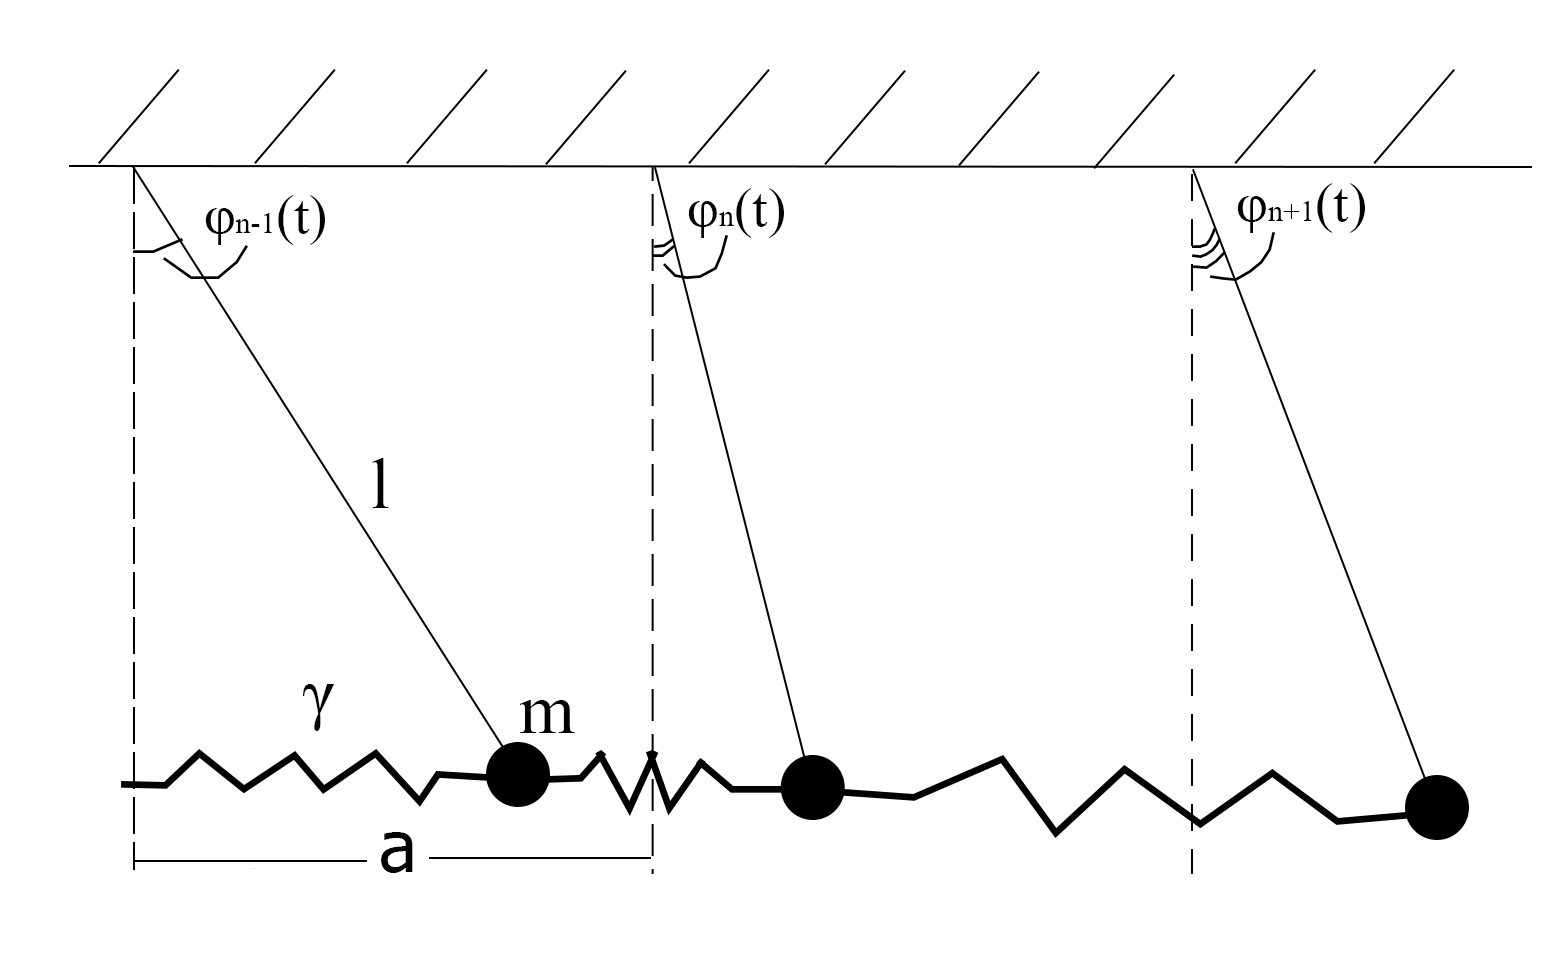
\includegraphics[width=0.5\linewidth]{fig/fig1.jpg}
	\label{fig:fig1}
\end{figure}

Состояние маятника зависит не только от времени t, но и от номера маятника n, т.е. n в некотором смысле играет роль пространственной координаты. Запишем уравнение динамики такого маятника:

\begin{equation}
	\ddot{\phi}_n+\omega^2_o \phi_n=\frac{\gamma}{m}[(\phi_{n-1}-\phi_n)+(\phi_{n+1}-\phi_n)].
	\label{eq:1}
\end{equation}

Каждый маятник действует на соседний, сила взаимодействия зависит от разности значений углов. Перепишем:

\begin{equation*}
	\ddot{\phi}_n+\omega^2_o \phi_n=\frac{\gamma}{m}[(\phi_{n-1}-2\phi_n+\phi_{n+1})].
\end{equation*}

Часто такую связь называют диффузионной, хотя, конечно, никакого отношения к процессу диффузии она не имеет. В системе нет диссипации, она линейна (нелинейность порождала бы новые частоты).

\begin{equation}
	\phi_n=A e^{i(\omega t-nka)}.
	\label{eq:2}
\end{equation}

Такая форма записи учитывает, что возмущение от маятника к маятнику проходит за некоторое конечное время.

\begin{equation*}
	-\omega^2+\omega_o^2=\frac{\gamma}{m}(e^{-ika}-2+e^{ika}),
\end{equation*}

\begin{equation}
	\omega^2=\omega_o^2-\frac{\gamma}{m}(e^{-ika}-2+e^{ika}).
	\label{eq:3}
\end{equation}

Рассмотрим случай \textit{k - действительное}
\begin{equation*}
	\omega^2=\omega_o^2-\frac{\gamma}{m}(-2+2\cos{ka}),
\end{equation*}

\begin{equation}
	\omega^2=\omega_o^2+\frac{4\gamma}{m}\sin^2{\frac{ka}{2}}.
	\label{eq:4}
\end{equation}

Установили, что $\omega$ и k связаны соотношением \eqref{eq:4}

\begin{figure}[H]
	\centering
	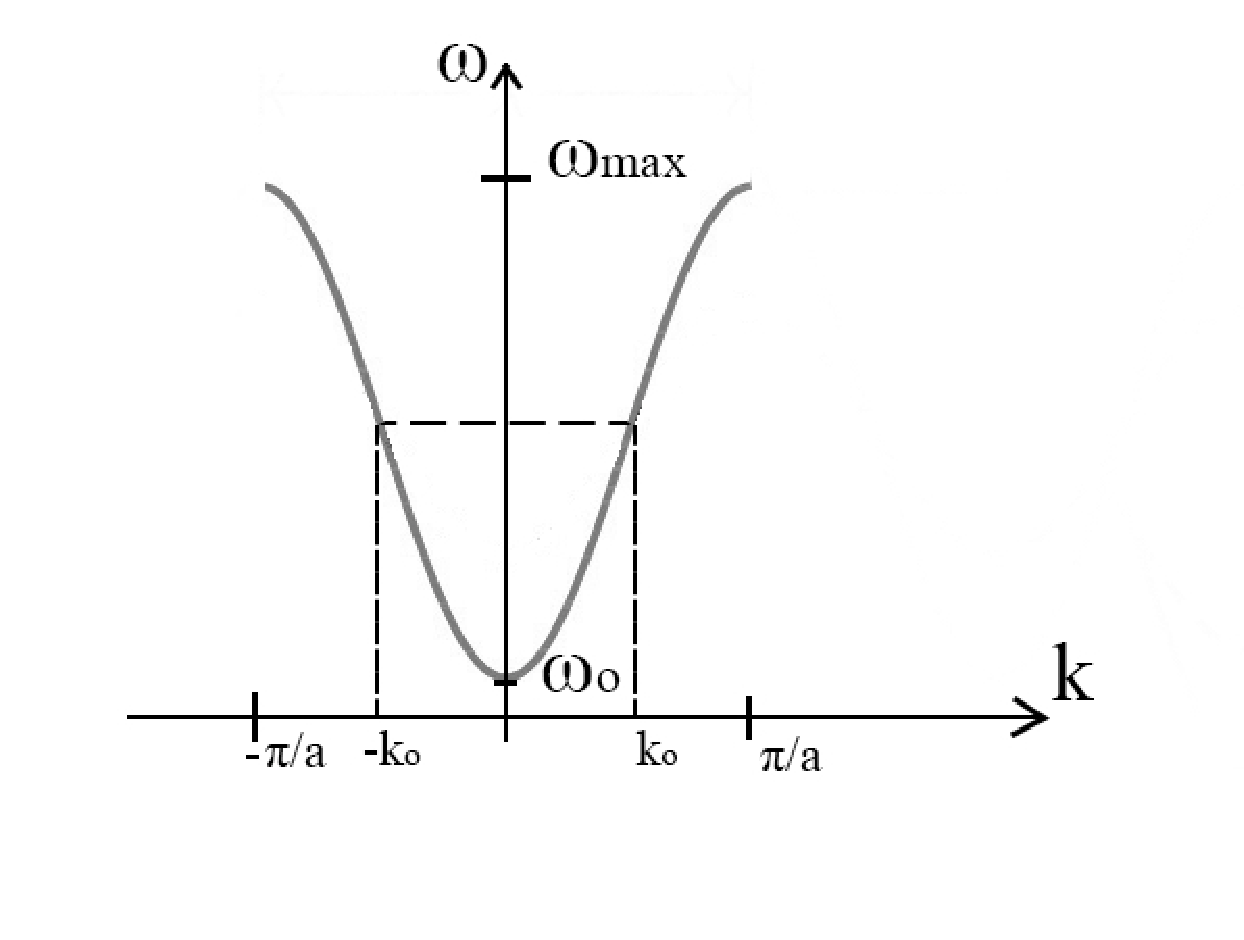
\includegraphics[width=0.5\linewidth]{fig/fig2.pdf}   
\end{figure}

\begin{equation*}
	\omega_{max}=\sqrt{\omega_o^2+\frac{4\gamma}{m}}.
\end{equation*}

Если $\omega_o < \omega < \omega_{max}$, то каждому $\omega$ соответствует $k_o$ и $-k_o$

Получим две гармонические бегущие волны:

\begin{equation*}
	\phi_n=A e^{i(\omega t+nk_oa)} ~~\text{и} ~~\phi_n=A e^{i(\omega t-nk_oa)},
\end{equation*}
где k - волновое число. Поскольку система линейна, любая линейная комбинация решений тоже будет решением. Диапазон $\omega_o < \omega < \omega_{max}$ называют полосой прозрачности (или полосой пропускания). Вне этой полосы решению не отвечают действительные k. В этом случае число \textit{k - чисто мнимое} (чисто - ибо нет диссипации в системе) и $k=i\kappa$:
\begin{equation}
	\omega^2=\omega_o^2-\frac{4\gamma}{m}\sh^2{\frac{\varkappa a}{2}},
	\label{eq:5}
\end{equation}
а $\phi_n=A e^{-n\varkappa a} e^{i\omega t}$ (при $n\rightarrow \infty$, $\phi_n \rightarrow 0$). В этих областях волна не проходит. 

Почему в одних случаях система пропускает волну, а в других нет?

Если мы находимся в полосе прозрачности, то $v_\text{фаз}=v_\text{фаз}(k), v_\text{фаз}=v_\text{фаз}(\omega)$. Если фазовая скорость зависит от частоты или волнового числа, то среда диспергирующая, а \eqref{eq:4} - дисперсионное соотношение. Дисперсия возникает из-за наличия собственных пространственно-временных масштабов (a и $\omega_o$). У каждой компоненты волнового пакета будет своя фазовая скорость, возникнет его деформация.

\subsection{Предельный переход от цепочной структуры в среде}
Введем пространственную координату $x$ вдоль балки. Сделаем замену, считая, что $\phi_n$ зависит от двух переменных:
\begin{gather*}
	\phi_n(t) \rightarrow \phi(x,t), \\
	\phi_{n+1}(t) \rightarrow \phi(x+a,t)=\phi(x,t)+\pdv{\phi}{x}a +\frac12 \pdv[2]{\phi}{x}a^2+\dots
\end{gather*}

Считая a малым, разложим в ряд по степеням a:

\begin{equation}
	\phi_{n-1}(t) \rightarrow \phi(x-a,t)=\phi(x,t)-\pdv{\phi}{x}a +\frac12 \pdv[2]{\phi}{x}a^2+\dots,
	\label{eq:6}
\end{equation}
и подставим в \eqref{eq:1}

\begin{gather*}
	\pdv[2]{\phi}{t} + \omega_o^2 \phi=\frac{\gamma}{m}a^2 \pdv[2]{\phi}{x}, \\
	\frac{\gamma}{m}a^2 = v^2,
\end{gather*}
\begin{equation}
	\pdv[2]{\phi}{t}-v^2\pdv[2]{\phi}{x}+\omega_o^2\phi=0 -\text{Уравнение Клейна-Гордона}.
	\label{eq:7}
\end{equation}

Уравнение \eqref{eq:7} не что иное, как уравнение в частных производных. Когда мы можем использовать \eqref{eq:7} вместо \eqref{eq:1}?

Предполагали, что
\begin{enumerate}
	\item $\phi_n$, определенная в точке, определена и между дискретными точками подвеса;
	\item отброшены величины третьего порядка;
	\item a-мало
\end{enumerate}

Построим дисперсионную характеристику для \eqref{eq:7}

\begin{gather*}
	\phi(x,t)=Ae^{i(\omega t + kx)}, \\ -\omega^2-k^2v^2+\omega_o^2=0,
\end{gather*}
\begin{equation}
	\omega^2 = \omega_o^2 + k^2v^2.
	\label{eq:8}
\end{equation}
\begin{figure}[H]
	\centering
	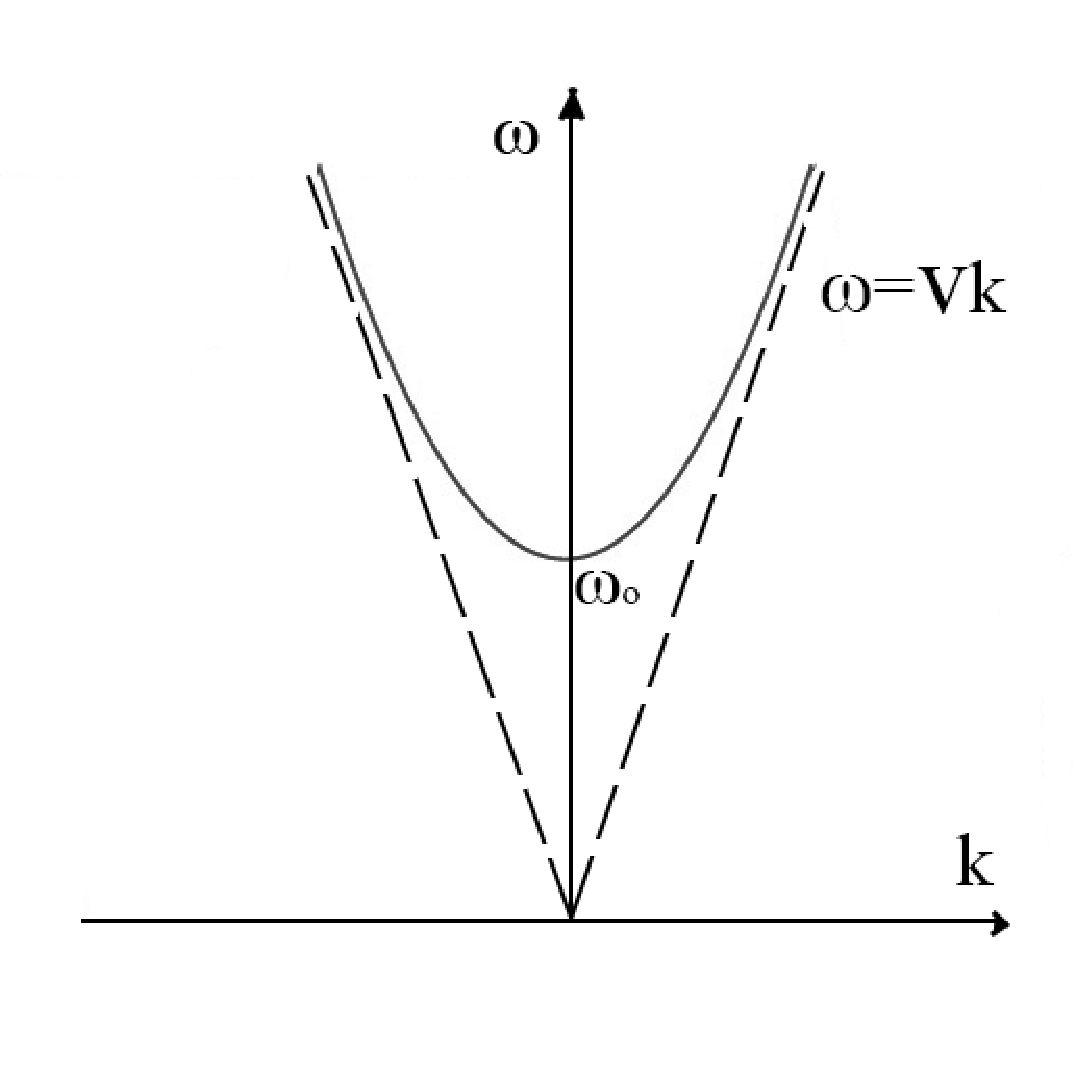
\includegraphics[width=0.5\linewidth]{fig/fig3.pdf}   
\end{figure}

Есть две асимптоты. 

При каких условиях дисперсионки совпадут?

$\lambda\gg a$ или $ka\ll$ - условие длинноволновой зоны, можно от одной перейти к другой, поскольку пространственный масштаб не сказывается, мы им пренебрегаем. Если $\omega_0 \rightarrow 0$, то из \eqref{eq:8}: $\omega^2=k^2v^2$. В этом случае система не обладает дисперсией. 

\begin{figure}[H]
	\centering
	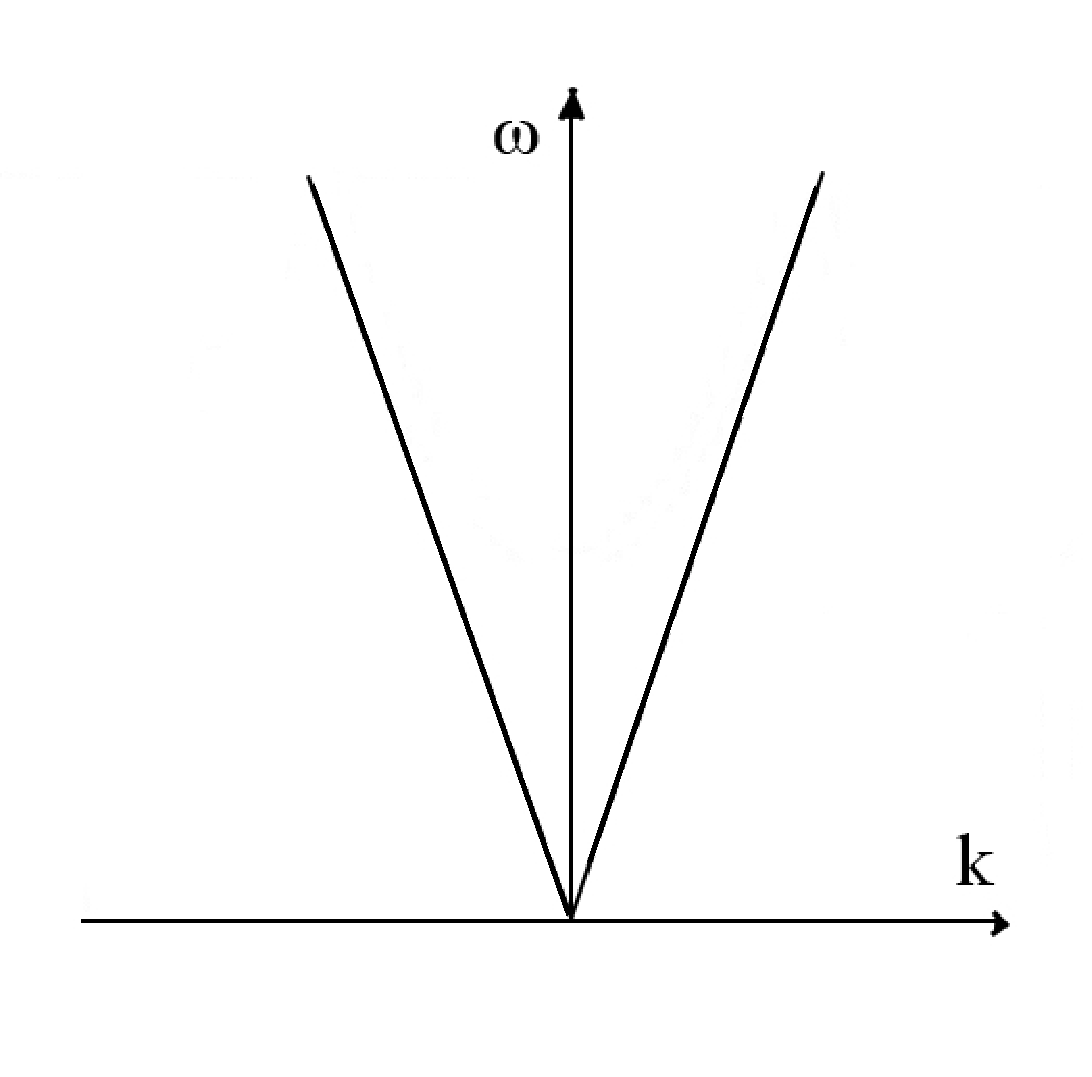
\includegraphics[width=0.5\linewidth]{fig/fig4.pdf}   
\end{figure}

Дисперсионная характеристика проявляется в области прозрачности/непрозрачности и зависимости $v_\text{фаз}$ от k или $\omega$.

Получили, шарики плотно друг к другу и покоятся.

Переход от цепочки к среде называется длинноволновым переходом. при нем теряется дискретность системы.

\subsection{Составление дисперсионного уравнения для произвольной линейной системы}

Рассмотрим многомерную систему
\begin{equation}
	A\pdv{\vec{U}}{t}+B\pdv{\vec{U}}{x}+C\vec{U}=0.
	\label{eq:9}
\end{equation}

A, B, C - $n\times n$ - матрицы; $\vec{U}(x,t)$ описывает состояние системы.

\begin{equation}
	\vec{U}=\vec{\phi} e^{i(\omega t - kx)}.
	\label{eq:10}
\end{equation}

\begin{equation*}
	\vec\phi=
	\begin{pmatrix}
		\phi_1 \\
		\phi_2 \\
		\phi_3 \\
		\vdots \\
		\phi_n \\
	\end{pmatrix}
	,
\end{equation*}

\begin{equation*}
	Ai\omega\vec\phi-iBk\vec\phi+C\vec\phi=0,
\end{equation*}
\begin{equation}
	(A\omega-Bk-iC)\vec\phi i=0.
	\label{eq:11}
\end{equation}

\eqref{eq:11} представляет собой систему линейных однородных уравнений относительно компонент вектора $\vec\phi$. Она имеет решение, если ее детерминант
\begin{equation}
	det(A\omega-Bk-iC)=0.
	\label{eq:12}
\end{equation}

для краткости обозначают $D(\omega,k)=0$. он связывает $\omega$ и k, т.е. задает дисперсионную характеристику. Следовательно, для $\forall k$ дисперсионное соотношение определяют n значений $\omega$: $\omega_1(k), \dots, \omega_n(k)$. Каждой паре k, $\omega_s(k)$ отвечает некоторый вектор, определяемый \eqref{eq:11}. При этом решением будут не только $k, \omega, \vec\phi$, но и $k^*, \omega^*, \vec\phi^*$. Можно построить действительное решение:
\begin{equation}
	\vec{U}(x,t)=\vec\phi e^{i(\omega t-kx)}+\vec\phi^* e^{-i(\omega^* t-k^*x)}.
	\label{eq:13}
\end{equation}

\eqref{eq:13} задает гармоническую волну, если $k, \omega$ действительные. Если же $k, \omega$ комплексные, то \eqref{eq:13} задает нарастающее или затухающее колебание. При этом общее решение может выть записано в виде 
\begin{equation*}
	\vec{U}(x,t)=\sum_{s=1}^{n} \phi^{(s)}e^{i(\omega_s(k)t-kx)} + \text{к.с}.
\end{equation*}

Как только будут учтены граничные условия, получится аналог характеристического уравнения.

\subsection{Влияние граничных условий}
Предположим, маятники были свернуты в кольцо, следовательно, должно уложиться целое число полуволн: 

\begin{gather*}
	n=1,\dots,N;~~\phi_{n-1}-2\phi_n+\phi_{n+1}; \\
	k=\frac{2\pi n}{l};~~\phi_{N+1}=\phi_1;~~k=k_n.
\end{gather*}	

Примером распределенной системы может служить струна длины l, концы которой закреплены:
\begin{figure}[H]
	\centering
	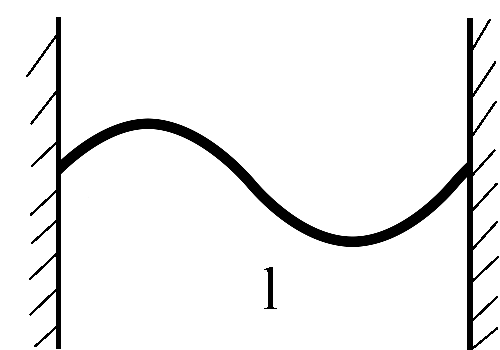
\includegraphics[width=0.5\linewidth]{fig/fig5.pdf}   
\end{figure}
\begin{gather*}
	U(x,t), \\ U(0,t)=u(l,t)=0, \\ U(x,t)=\phi_1 e^{i(\omega t-kx)}+\phi_2 e^{i(\omega t+kx)}, \\
	\begin{cases}
		\phi_1 e^{i\omega t}+\phi_2 e^{i\omega t}=0 \\
		\phi_1 e^{i\omega t}+\phi_2 e^{i\omega t+ikl}=0
	\end{cases}
	\\ \phi_1=-\phi_2,~~ \sin{kl}=0,~~ k=\frac{\pi n}{l}=k_n
\end{gather*}

\begin{equation}
	\begin{cases}
		D(\omega,k)=0 \\
		k=k_n
	\end{cases}
	\label{eq:14}
\end{equation}

Отсюда следует, что $\omega=omega_n$. Если среда без дисперсии, то спектры волновых чисел и волновых частот будут эквидистантными. 

\subsection{Устойчивость состояний равновесия нелинейных распределенных систем}
Простейшим типом решений распределенных систем являются такие состояния, которые не меняются ни во времени, ни в пространстве: $U(x,t); U=U_o=const$.
\begin{equation}
	\pdv{U}{t}=f(U)+D\pdv[2]{U}{x},
	\label{eq:15}
\end{equation}
где $f(U)$ - нелинейная функция. Пусть, кубическая. Если убрать D. то уравнение будет описывать динамику точки в среде.
\begin{figure}[H]
	\centering
	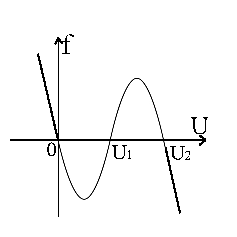
\includegraphics[width=0.5\linewidth]{fig/fig6.pdf}   
\end{figure}

Три точки, где $f(U)=0$. В системе могут быть стационарные решения (не зависящие от времени) - это другой тип решения. Будем рассматривать их решение в классе гармонических функций. 
\begin{equation*}
	\xi(x,t) \sim e^{pt+ikx}
\end{equation*}

Линеаризуем \eqref{eq:15} на состояниях равновесия:
\begin{equation*}
	U=U^*+\xi(x,t),
\end{equation*}
\begin{equation}
	\pdv{\xi}{t}=D\pdv[2]{\xi}{x}+f'(U^*)\xi(x,t).
	\label{eq:16}
\end{equation}
\begin{gather*}
	f(U^*+\xi(x,t))\approx f(U^*)+f'(U^*)\cdot\xi(x,t), \\ \xi(x,t)=A e^{pt+ikx} \\
	p =-Dk^2+f'(U^*), \\ U=0,~~U=U_2,~~f'(U^*)<0.
\end{gather*}

Для каждого А.
\begin{figure}[H]
	\centering
	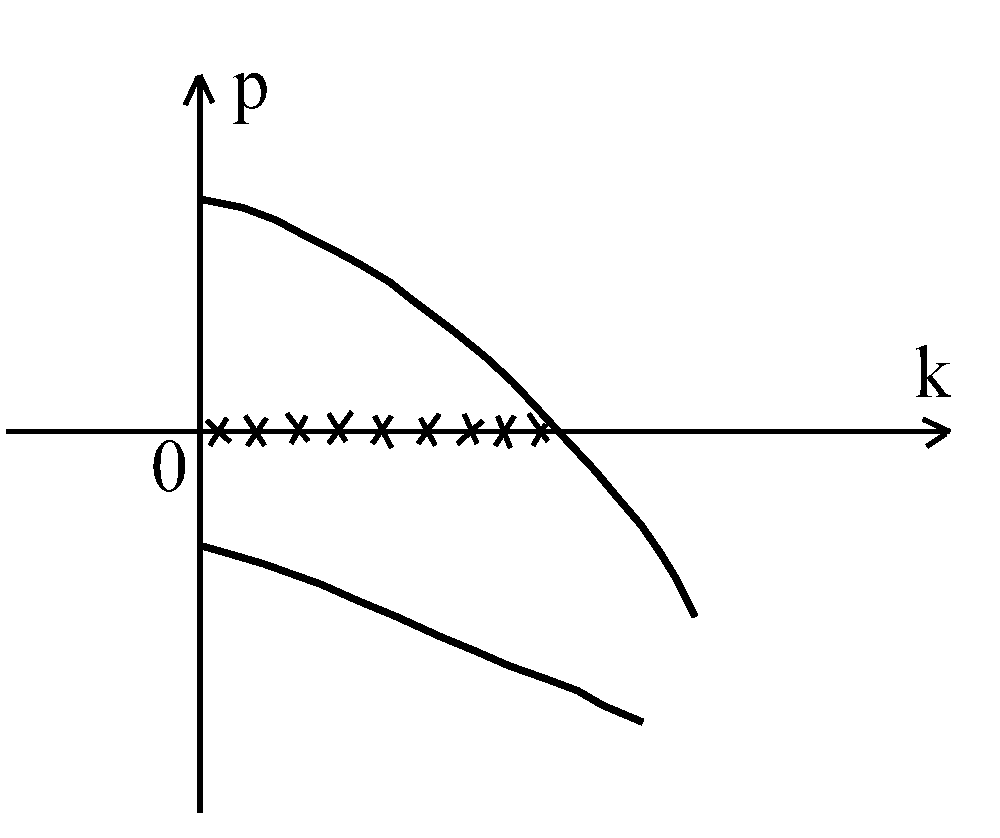
\includegraphics[width=0.5\linewidth]{fig/fig7.pdf}   
\end{figure}

Все решения такого вида затухают, следовательно, $U=0, U=U_2$ устойчивые, а $U_1$ - неустойчивое в классе возмущений $\xi(x,t)=A e^{pt+ikx}$.

В частности, \eqref{eq:15}, описывает распространение пламени по бикфордовому (огнепроводному) шнуру. Волна превращает вещество из несгоревшего материала в сгоревшее.


\section{15.04.19 Диффузионная неустойчивость. Структура Тьюринга}
Многие биологические объекты обладают периодической структурой. Например, зебра, дождевой червь, сороконожка. Однако известно, что изначально, при появлении, они однородны. Рассмотрим одномерный случай структур.

Тьюринг предположил, что существуют два вещества. Одно из них - $U(x,t)$ - стимулирует рост клеток. Его назвали активатором. Другое - $V(x,t)$ - замедляет рост. Это ингибитор. Следующим предположением было наличие некоторых химических реакций и присутствие диффузии. Фактически, Тьюринг записал уравнение реакции диффузии. 
\begin{equation}
\begin{cases}
		\pdv{U}{t}=f(U,V)+D_1 \pdv[2]{U}{x} \\
		\pdv{V}{t}=g(U,V)+D_2 \pdv[2]{V}{x},
	\end{cases}	\
	\label{eq:17}
\end{equation}
где $f,g$  - это некоторые нелинейные функции.

Эта система двухкомпонентная, произвольная координата одна. Предположим, \eqref{eq:17} имеет состояние равновесия, т.е. существует решение системы
\begin{equation}
\begin{cases}
		f(U,V)=0 \\
		g(U,V)=0.
	\end{cases}	\
	\label{eq:18}
\end{equation}
$U=U_0, V=V_0$.

Исследуем на устойчивость. Положим,
\begin{gather*}
	U=U_0+\xi(x,t) \\
	V=V_0+\eta(x,t).
\end{gather*}

Линеаризуем (оставляем только линейную часть):
\begin{equation}
	\begin{cases}
		\pdv{\xi}{t}=f'_u(U_0, V_0)\xi(x,t)+f'_v(U_0, V_0)\eta(x,t)+D_1 \pdv[2]{\xi(x,t)}{x} \\
		\pdv{\eta}{t}=g'_u(U_0, V_0)\xi(x,t)+g'_v(U_0, V_0)\eta(x,t)+D_2 \pdv[2]{\eta(x,t)}{x}.
	\end{cases}	
	\label{eq:19}
\end{equation}

Получили уравнения в частных производных. Будем искать решение в виде:
\begin{equation}
	\xi(x,t)=A e^{pt+ikx};~~\eta(x,t)=B e^{pt+ikx}.
	\label{eq:20}
\end{equation}

Подставляя эти решения и учитывая, что $f'$ и $g'$ - это производные в точке, т.е. константы, получим:
\begin{equation}
	\begin{cases}
		\pdv{\xi}{t}=a\xi+b\eta+D_1 \pdv[2]{\xi}{x} \\
		\pdv{\eta}{t}=c\xi+d\eta+D_2 \pdv[2]{\eta}{x},
	\end{cases}	
	\label{eq:20}
\end{equation}
где
\begin{gather*}
	a=f'_u(U_0, V_0),~~b=f'_v(U_0, V_0),~~c=g'_u(U_0, V_0),~~d=g'_v(U_0, V_0).
\end{gather*}

\begin{equation}
	\begin{cases}
		Ap=aA+bB-k^2 D_1A \\
		Bp=cA+dB-k^2 D_2A,
	\end{cases}	
	\label{eq:21}
\end{equation}

\eqref{eq:17} представляет собой систему линейных однородных уравнений относительно констант А,В. Она имеет нетривиальное решение, если ее определитель не равен нулю. Раскрывая определитель, получим характеристическое уравнение для p:
\begin{equation}
	p^2+(D_2k^2+D_1k^2-a-d)p+(D_1k^2-a)(D_2k^2-d)-bc=0.
	\label{eq:22}
\end{equation}

Предположим, что в начальный момент $D_1=D_2=0$, тогда
\begin{equation}
	p^2-(a+d)p+ad-bc=0.
	\label{eq:23}
\end{equation}

Сначала структуры у животных нет, следовательно, без диффузии имеем устойчивое равновесие. Запишем условие для этого:
\begin{gather*}
	\Delta_o=ad-bc>0, \\ \sigma_0=a+d<0,
\end{gather*}
тогда состояние равновесия будет устойчивым. 

\begin{figure}[H]
	\centering
	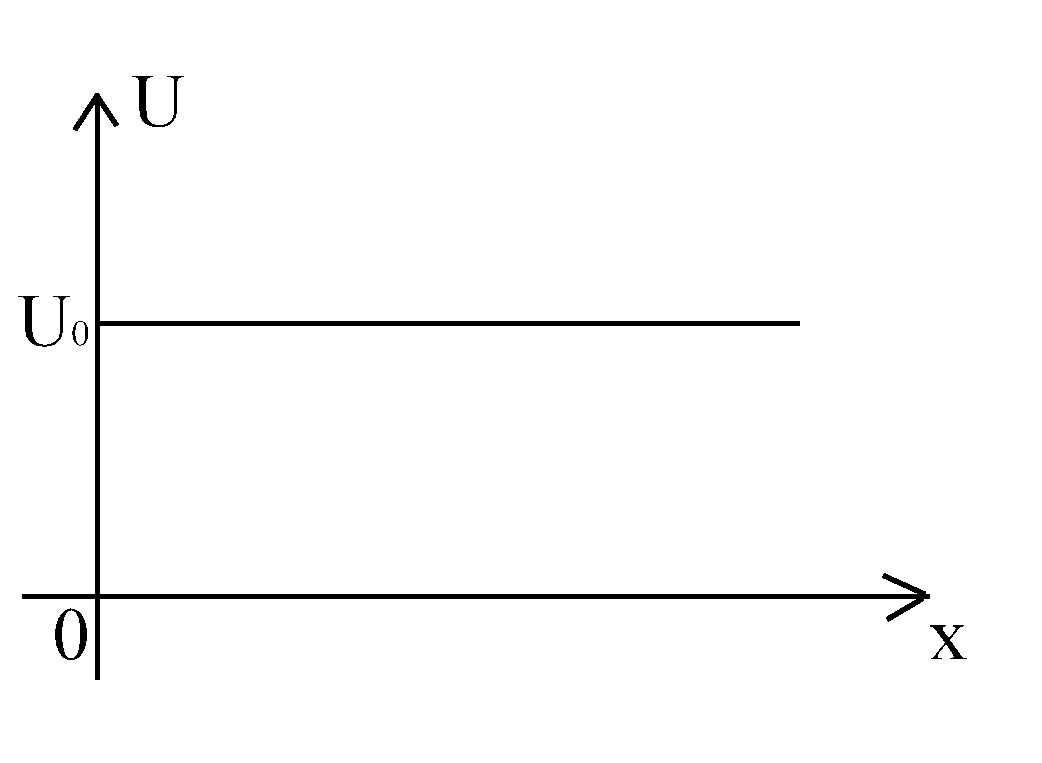
\includegraphics[width=0.5\linewidth]{fig/fig8.pdf}   
\end{figure}

По оси х U(активатор) и V(ингибитор) постоянны. 

Пусть теперь $D_1, D_2 \neq 0$. В этом случае \eqref{eq:23} после преобразований примет вид:
\begin{equation*}
	p^2-\sigma p+\Delta=0,
\end{equation*}
где
\begin{gather*}
	\Delta=a+d-(D_1+D_2)k^2=\sigma_0-(D_1+D_2)k^2, \\ \sigma=ad-bc-(aD_2+dD_1)k^2+D_1D_2k^4=\Delta_0-(aD_2+dD_1)k^2+D_1D_2k^4.
\end{gather*}

$Re\{p\}$ зависит от k. Анализ показывает:
\begin{figure}[H]
	\centering
	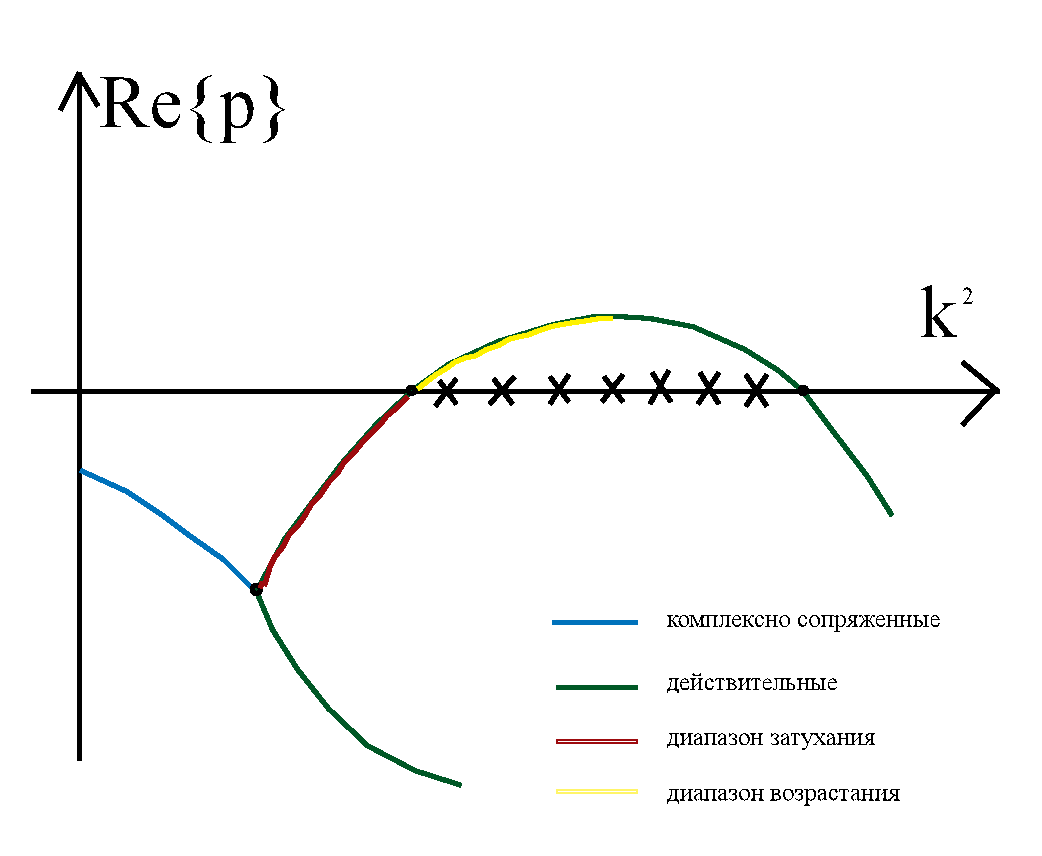
\includegraphics[width=0.5\linewidth]{fig/fig9.pdf}   
\end{figure}

Есть диапазон, где произошла потеря устойчивости состояния равновесия за счет действия диффузии. Это называется диффузионной неустойчивостью. Возникает аналог бифуркации Андронова-Хопфа. В диапазоне затухания все моды затухают, а возрастания - возрастают. Возникает периодическое по пространственной координате решение. Кроме того, оно пространственно неоднородное.  
\begin{figure}[H]
	\centering
	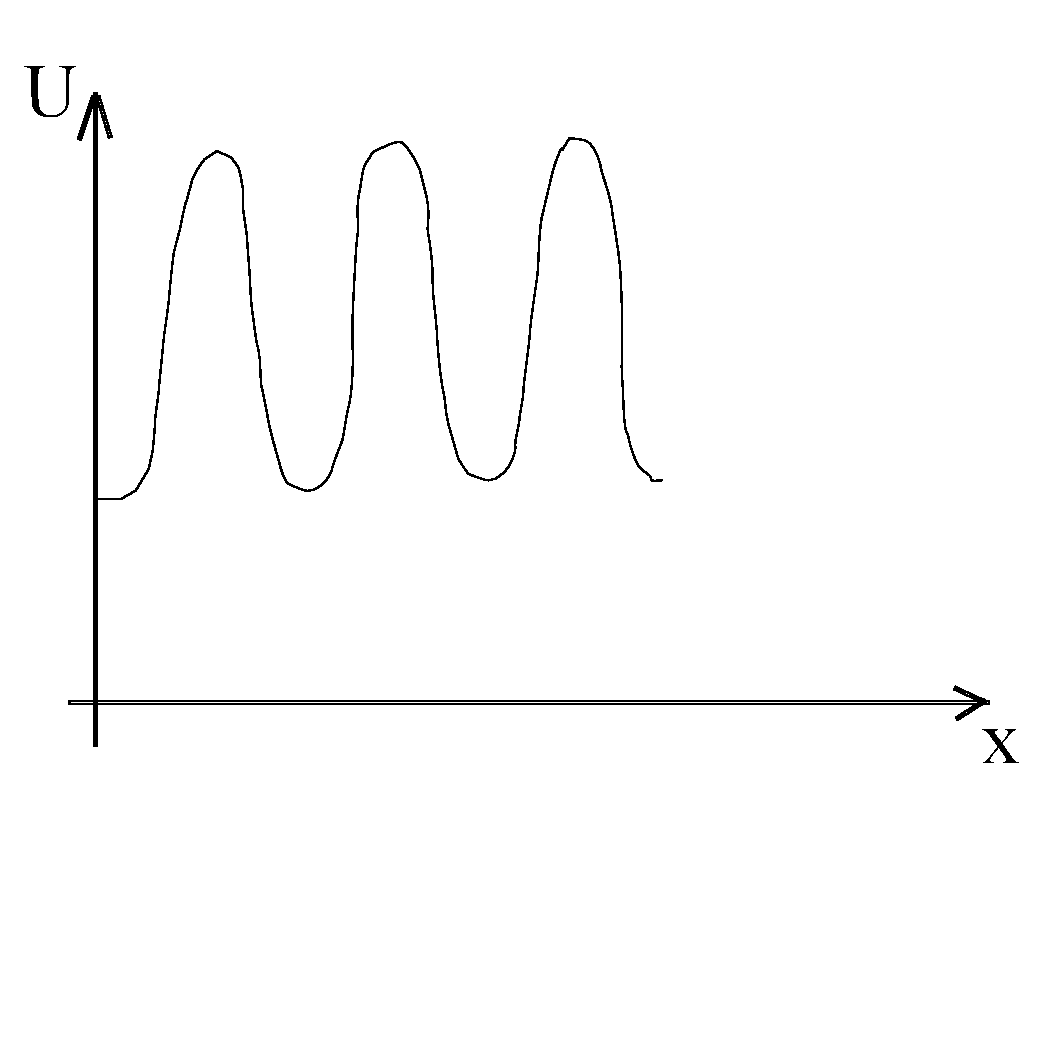
\includegraphics[width=0.5\linewidth]{fig/fig10.pdf}   
\end{figure}

Динамическая структура, обладающая свойством структурной устойчивости, иногда называется диссипативной структурой. Возникает за счет баланса. 

\subsection{Простые волны. Образование разрывов.}
Рассмотрим равномерную среду, свойства которой описывает скалярная функция $U(x,t)$. Среда линейная, без дисперсия. В таких средах возможно существование волновых движений, при этом все переменные описываются одинаковыми уравнениями:
\begin{equation}
	\pdv{U_j}{t}+V\pdv{U_j}{x}=0.
	\label{eq:24}
\end{equation}

В среде нет собственных масштабов и нелинейностей. V-const. В этой среде возможно существование так называемых римановых волн. 
\begin{equation*}
	U_j=\phi(x-Vt),
	\label{eq:25}
\end{equation*}
где $\phi$ - произвольная, обязательно дифференцируемая, функция.

Введем бегущую координату:
\begin{gather*}
	\xi=x-Vt, \\ \dv{\phi}{\xi} \pdv{\xi}{t}+V\dv{\phi}{\xi} \pdv{\xi}{x}=0, \\ -V\dv{\phi}{\xi}+V\dv{\phi}{\xi} \equiv 0.
\end{gather*}

\eqref{eq:25} является решением такой системы. 

Теперь рассмотрим нелинейную среду (но все еще без дисперсии). В таких средах могут существовать волны, которые обладают следующим свойством: переменные связаны алгебраически (если есть $U_1$ и $U_2$, то $U_3$ всегда можно пересчитать).

Рассмотрим пример: волны на мелкой воде. Гравитационные волны вдоль оси x.
\begin{figure}[H]
	\centering
	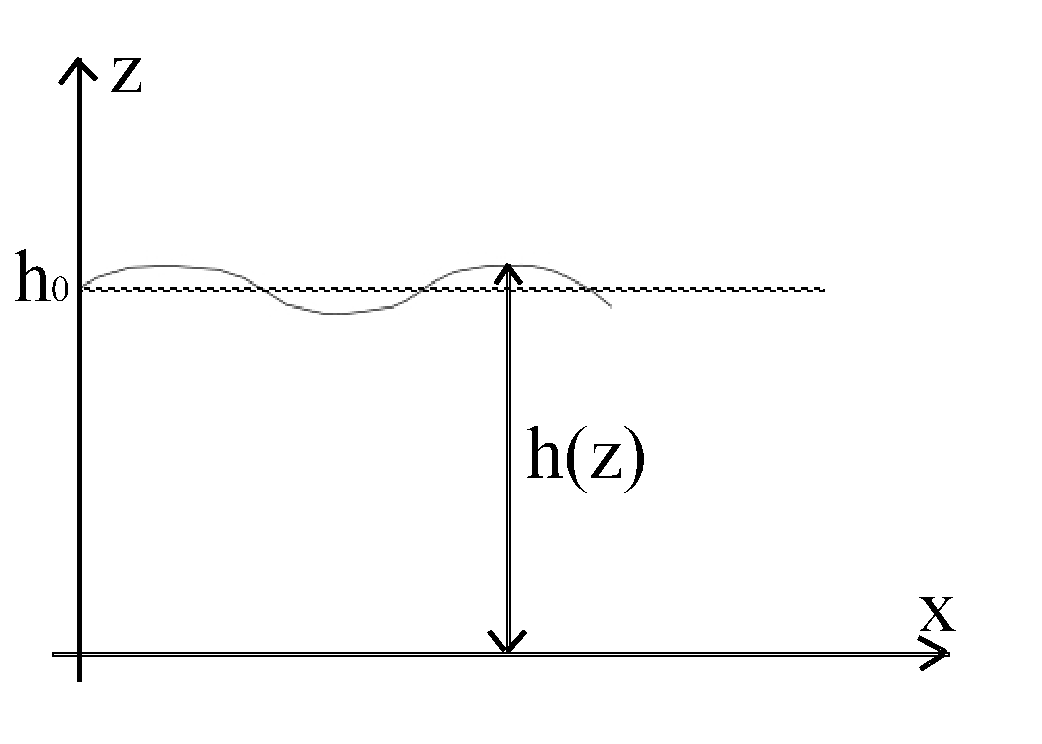
\includegraphics[width=0.4\linewidth]{fig/fig11.pdf}   
\end{figure}
$\lambda \gg h_0$

Состояние жидкости описывается: V - скоростью волны, h - профилем. Поскольку волны длинные, считаем, что $V\neq V(z)$.

Используем уравнение Эйлера: 
\begin{gather*}
	\pdv{V}{t}+V\pdv{V}{x}+\frac1{\rho}\pdv{\rho}{x}=0, \\ \rho=const, p-\text{среднее по высоте}, \\ \frac1{\rho}\pdv{\rho}{x}=g\pdv{h}{x}.
\end{gather*}

Давление больше там, где выше жидкость.
\begin{equation}
	\pdv{V}{t}+V\pdv{V}{x}+g\pdv{h}{x}=0.
	\label{eq:26}
\end{equation}

Добавим уравнение непрерывности:
\begin{gather*}
	\pdv{p}{t}+\pdv{(Vh)}{x}=0. 
\end{gather*}

Скорость изменения высоты слоя связана с разностью потока через x и dx
\begin{equation}
	\pdv{h}{t}+V\pdv{h}{x}+h\pdv{V}{x}=0.
	\label{eq:27}
\end{equation}

Предположим, h и V не являются независимыми переменными и $h=h(V)$.

Из уравнения \eqref{eq:26}: 
\begin{gather*}
	\pdv{h}{x}=\dv{h}{V}\pdv{V}{x}, \\ \pdv{V}{t}+V\pdv{V}{x}+g\pdv{h}{x} = 0 ~(*).
\end{gather*}

Из уравнения \eqref{eq:27}:
\begin{gather*}
	\dv{h}{V}\pdv{V}{t}+V\dv{h}{V}\pdv{V}{x}+h(V)\pdv{V}{x} = 0, \\ \pdv{V}{t}+V\pdv{V}{x}+\frac{h(V)}{\dv{h}{V}}\pdv{h}{x} = 0 ~(**).
\end{gather*}

(*) и (**) должны совпадать, т.к описывают одну и ту же величину. 
\begin{equation*}
	g\dv{h}{V}=\frac{h}{\dv{h}{V}}~ \text{или} ~(\dv{h}{V})^2=\frac{h}{g} - \text{уравнение для нахождения h}.
\end{equation*}

\begin{gather*}
	\dv{h}{V}=\pm \sqrt{\frac{h(V)}{g}}, \\ \pdv{V}{t}+V\pdv{V}{x}\pm \sqrt{h(V)g} \pdv{V}{x} = 0.
\end{gather*}
\begin{equation}
	\pdv{V}{t}+(V\pm \sqrt{h(V)g})\pdv{V}{x} = 0
	\label{eq:28}
\end{equation}
- уравнение простой волны, которое в общем виде выглядит:
\begin{equation}
	\pdv{U}{t}+V(U)\pdv{U}{x} = 0
	\label{eq:29}
\end{equation}

Это уравнение справедливо не только на мелкой воде. Здесь $V$ - это функция среды.

Будем искать решение в виде:
\begin{equation}
	U = \phi(x-V(U)t),
	\label{eq:30}
\end{equation}
\begin{gather*}
	\xi=x-V(U)t.
\end{gather*}

Убедимся, что \eqref{eq:30} - решение:
\begin{gather*}
	\pdv{U}{t}=\dv{\phi}{\xi}\pdv{\xi}{t}=\dv{\phi}{\xi}\qty(-V(U)-t\dv{V}{U}\pdv{U}{t}), \\ \pdv{U}{t}\qty(1+\dv{\phi}{\xi}\dv{V}{U}t)=-V(U)\dv{\phi}{\xi},
\end{gather*}
\begin{equation}
	\pdv{U}{t}=-V(U)\dv{\phi}{\xi} \frac{1}{(1+\dv{\phi}{\xi}\dv{V}{U}t)}
	\label{eq:31}
\end{equation}
\begin{gather*}
	\pdv{U}{x}=\dv{\phi}{\xi} \frac{1}{(1+\dv{\phi}{\xi}\dv{V}{U}t)}
\end{gather*}

Для определенности:
\begin{figure}[H]
	\centering
	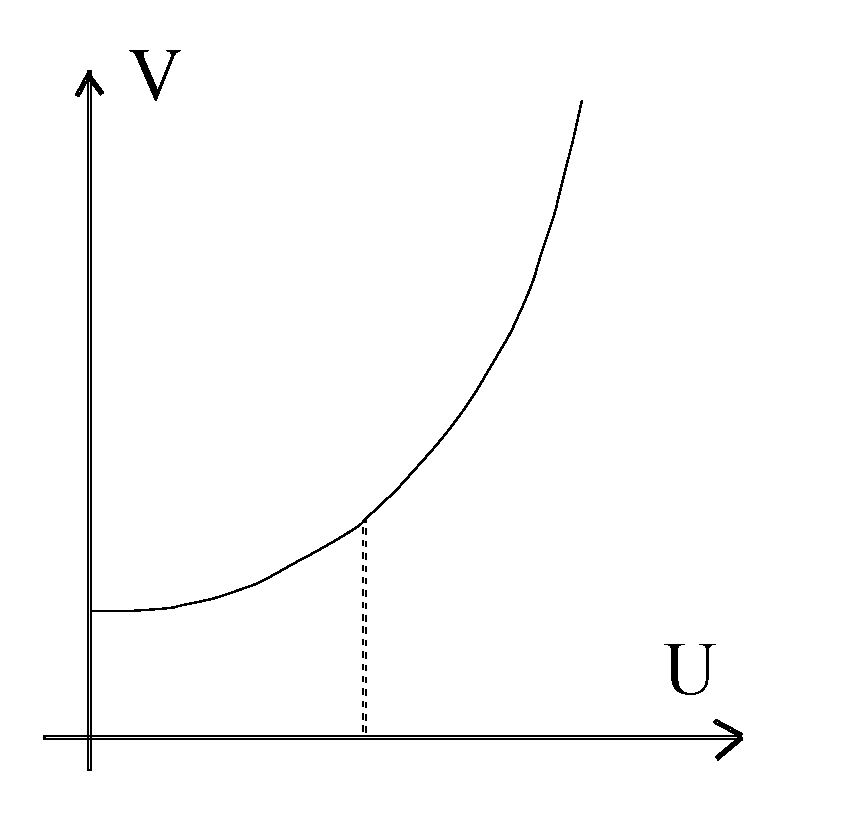
\includegraphics[width=0.4\linewidth]{fig/fig12.pdf}   
\end{figure}

У максимального значения U скорость наибольшая. Задается профиль $\phi$ при $t=0$:
\begin{figure}[H]
	\centering
	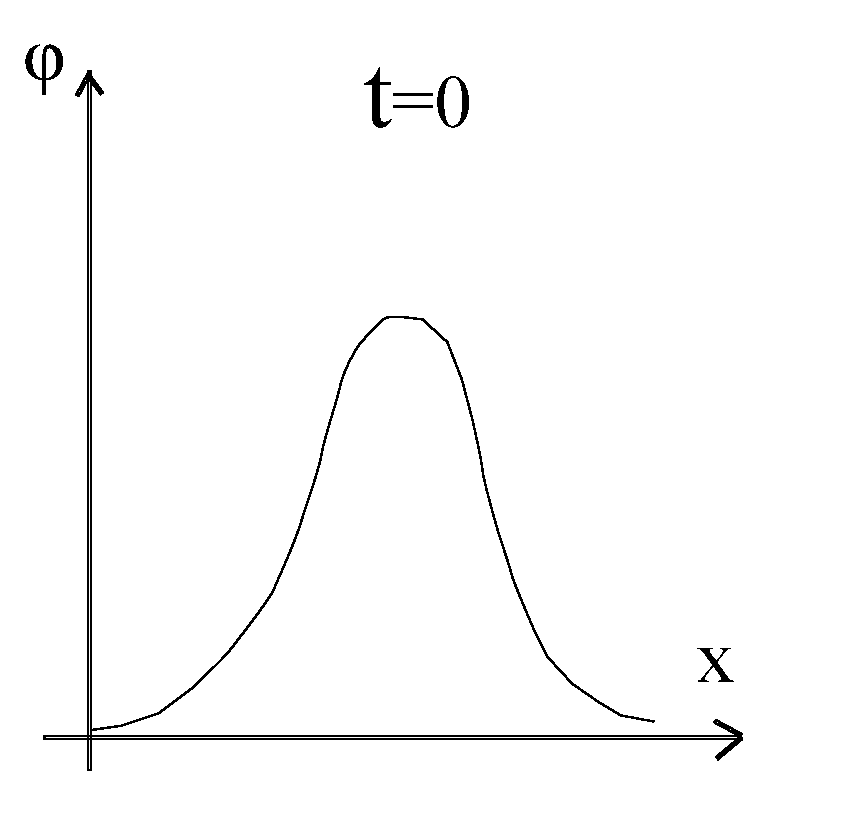
\includegraphics[width=0.4\linewidth]{fig/fig13.pdf}   
\end{figure}
или при $x=0$:
\begin{figure}[H]
	\centering
	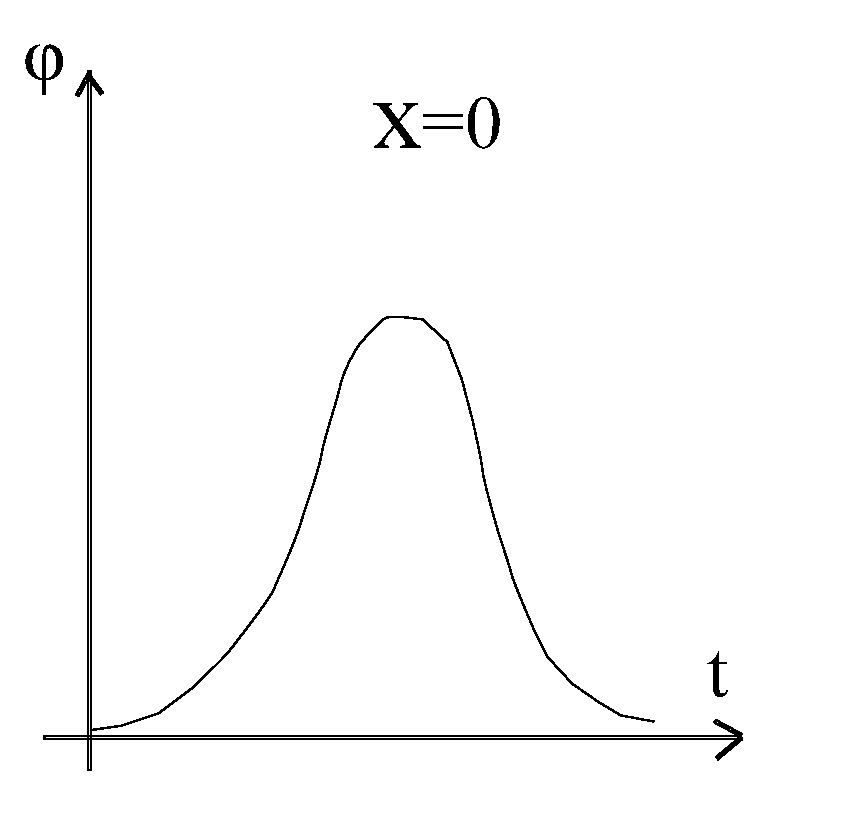
\includegraphics[width=0.4\linewidth]{fig/fig14.pdf}   
\end{figure}

Во время распространения, верх волны обгонит, произойдет укручение фронта, волна деформируется. 
\begin{figure}[H]
	\centering
	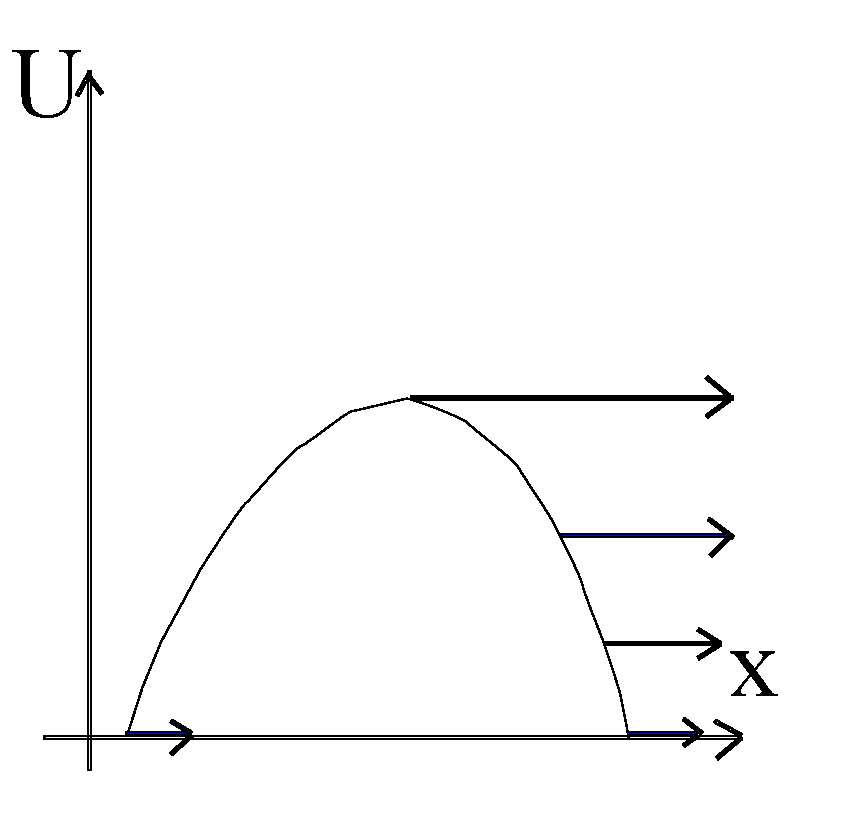
\includegraphics[width=0.4\linewidth]{fig/fig15.pdf}   
\end{figure}
\begin{figure}[H]
	\centering
	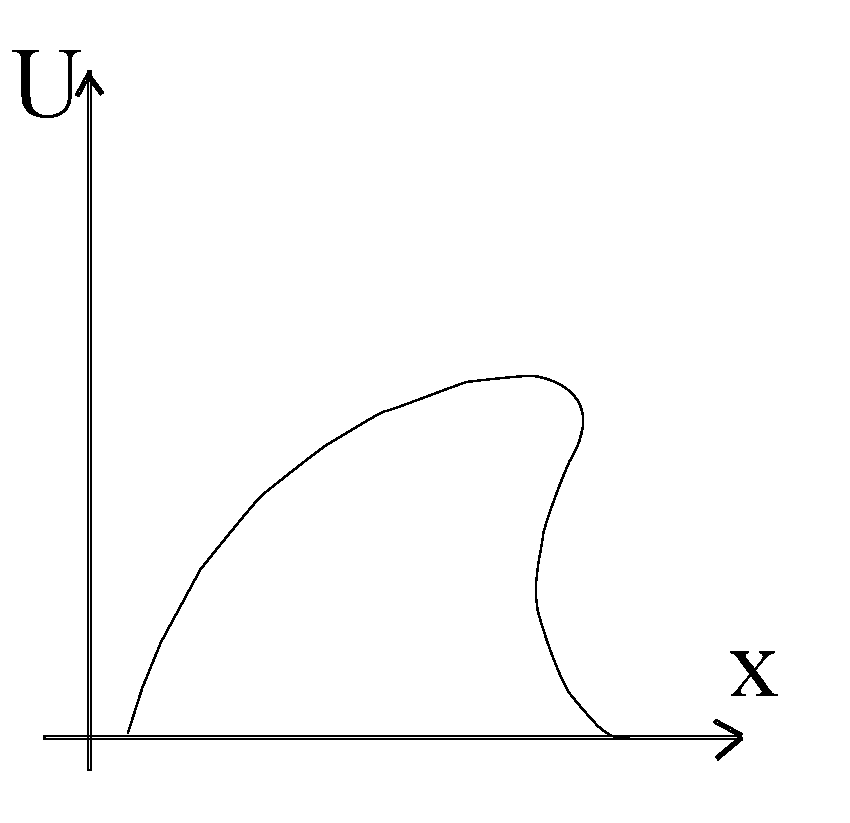
\includegraphics[width=0.4\linewidth]{fig/fig16.pdf}   
\end{figure}
\begin{figure}[H]
	\centering
	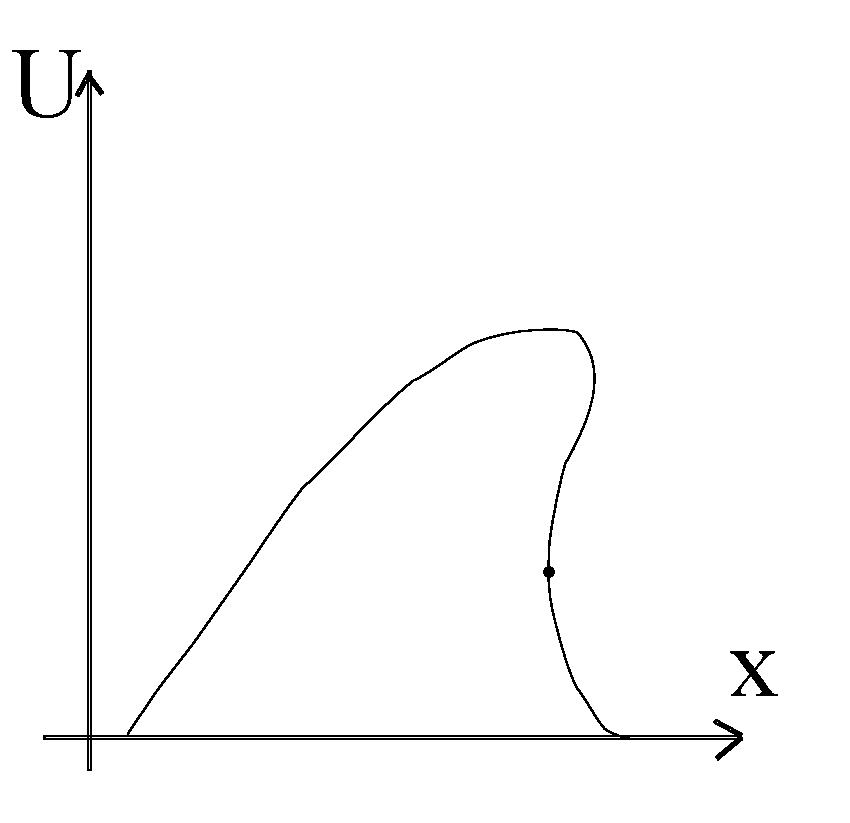
\includegraphics[width=0.4\linewidth]{fig/fig17.pdf}   
\end{figure}

Появится точка, где производные $\pdv{U}{t}, \pdv{U}{x} \rightarrow \infty $. Образуется бесконечный градиент и разрыв, который характеризуется состоянием $U^*, t^*, x^*$, его описание в рамках простой волны несправедливо. Вторые производные тоже обращаются в бесконечность, и точки эти можно найти.

\section{Солитоны в уравнении Кортевега - де Фриза} 
Рассмотрим узкий бассейн с жидкостью (должен быть достаточно длинным):
\begin{figure}[H]
	\centering
	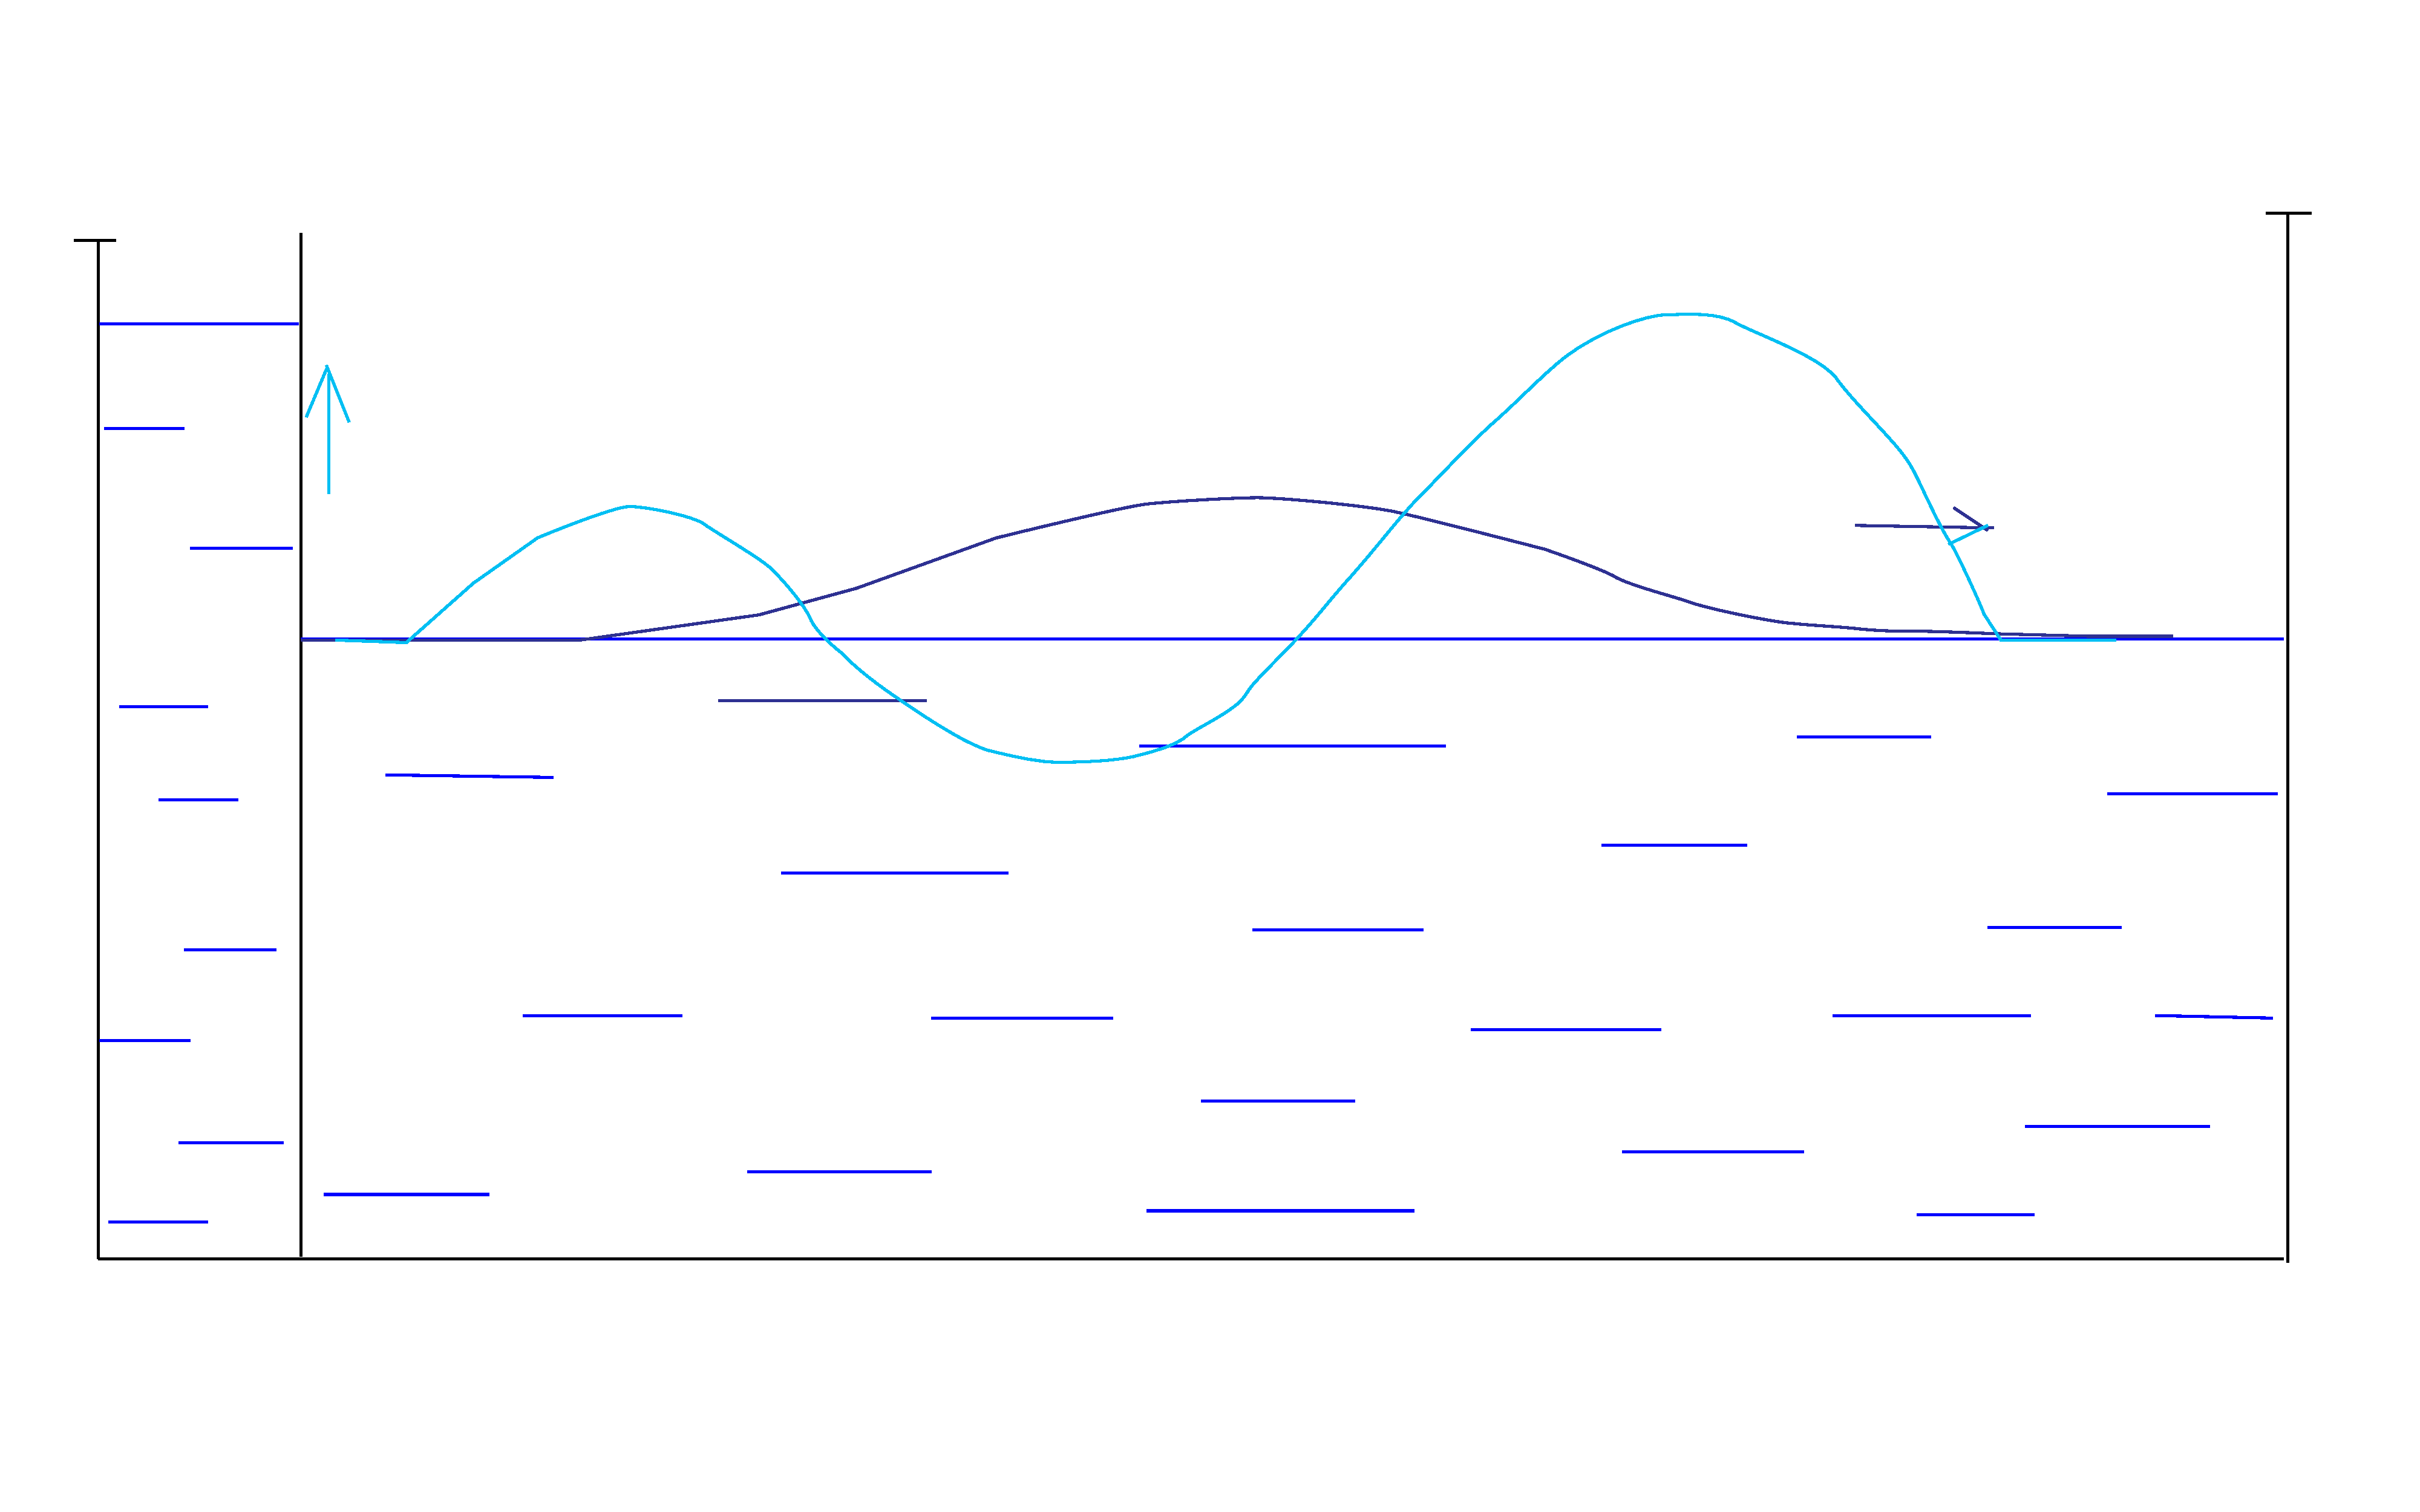
\includegraphics[width=0.4\linewidth]{fig/fig18.pdf}   
\end{figure}

Подбирают соотношение масс воды в емкостях. Резко поднимают задвижку. В зависимости от соотношения масс воды, могут побежать разные волны, разное количество холмов. 

Канал, который мы рассматриваем, мелкий, средней глубины $l$; $l+\eta(x,t)$. Поверим на слово: 
\begin{equation*}
	\pdv{\eta}{t}=\frac32 \sqrt{\frac{g}{l}}\pdv{}{x}\qty(\frac32 \alpha \eta+\frac12 \eta^2+\frac13 \sigma \pdv[2]{\eta}{x}),
\end{equation*}
где $\sigma=\frac{l^3}{3}-\frac{Tl}{\rho g}$, $\alpha$-произвольная константа, $T$ - коэффициент поверхностного натяжения, $\rho$ - плотность жидкости.

Преобразовав, получим
\begin{equation}
	\pdv{U}{t}+U\pdv{U}{x}+\beta \pdv[3]{U}{x}=0.
	\label{eq:32}
\end{equation}
$\beta$ - некоторая константа, а последнее слагаемое характеризует дисперсию. Видно, что уравнение простой волны дополняется дисперсией. (К экзамену построить дисперсионную характеристику). 

Пусть есть квадратичная среда, в нее запускают волну $e^{i(\omega_o t+kx)}$. Среда нелинейная и без дисперсии. При таких условиях квадратичная среда порождает новые частоты. $\omega_o$ порождает $2\omega_o$. Если нет дисперсии, то нет пространственных масштабов. $2\omega_o$ порождает $3\omega_o$ и так далее, лавинно. Спектр стремится в бесконечность. 
\begin{figure}[H]
	\centering
	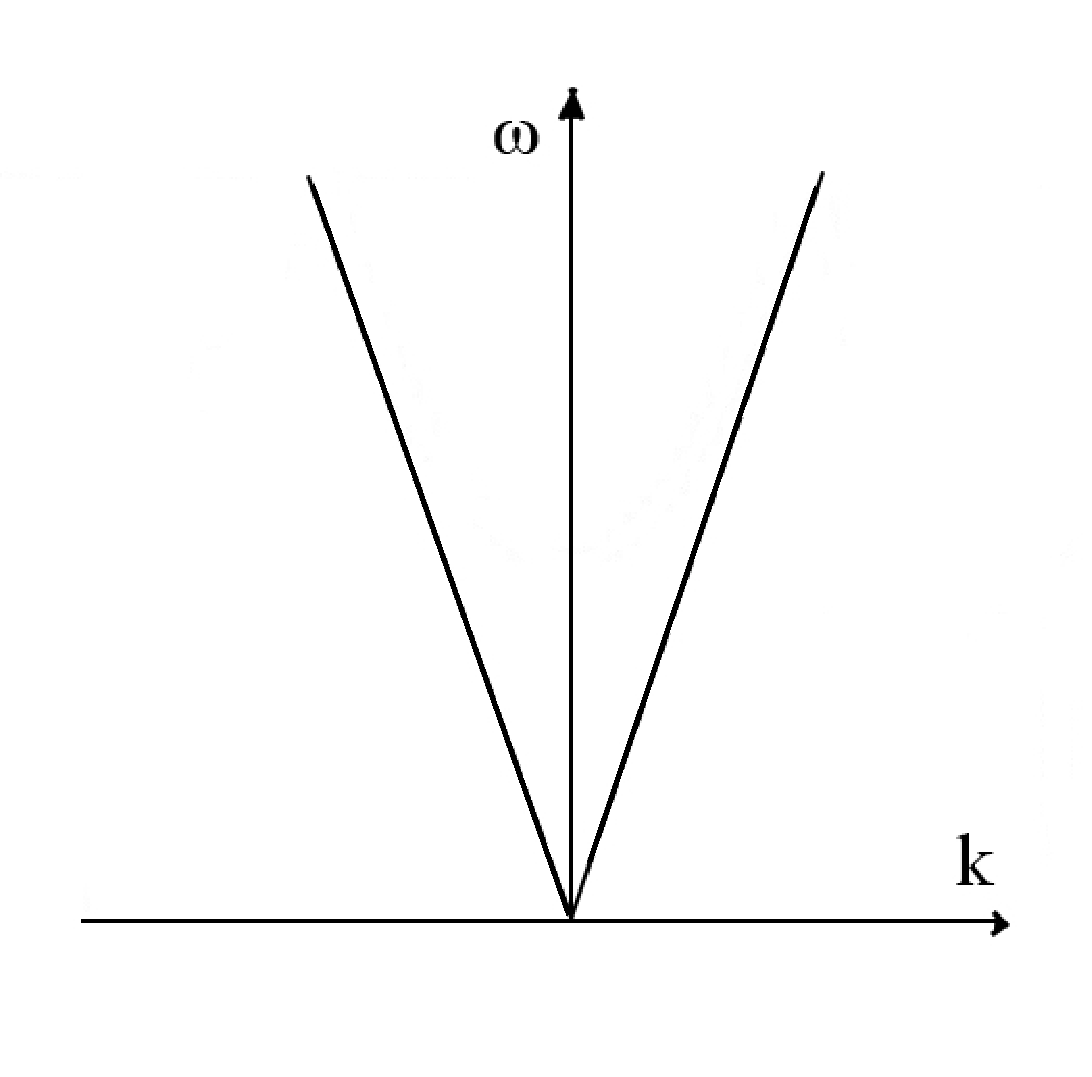
\includegraphics[width=0.4\linewidth]{fig/fig4.pdf}   
\end{figure}

Теперь включим дисперсию (в данном случае - высокочастотную). Она ограничивает частотный рост и стабилизирует волну. 

Будем искать решение уравнения \eqref{eq:32} в виде $U=U(x-Vt)$:
\begin{equation}
	-\pdv{U}{\xi}+U\pdv{U}{\xi}+\beta \pdv[3]{U}{\xi}=0.
	\label{eq:33}
\end{equation}

Интегрируя:
\begin{equation}
	\beta \pdv[2]{U}{\xi}+\frac{U^2}{2}-VU=0.
	\label{eq:34}
\end{equation}

Это есть уравнение нелинейного осциллятора. Для простоты константу интегрирования приравняли  к нулю, что дает уровень, откуда изменяется $U(x,t)$.
\begin{equation}
	\begin{cases}
		\dot{U}=y \\
		\beta \dot{y} =VU-\frac{U^2}{2}.		
	\end{cases}
	\label{eq:34}
\end{equation}

Получили систему для нелинейного осциллятора.
\begin{gather*}
	\beta \frac{y^2}{2}+E_{\text{п}} = const, \\ E_{\text{п}} = \frac{U^3}{6}-V\frac{U^2}{2}
\end{gather*}






\end{document}{}